%--------------------
% Packages
% -------------------
\documentclass[11pt,a4paper]{report}
\usepackage[utf8]{inputenc}
\usepackage[T1]{fontenc}
%\usepackage{gentium}
\usepackage{mathptmx} % Use Times Font

\usepackage[pdftex]{graphicx} % Required for including pictures
\usepackage[english]{babel} % Swedish translations
\usepackage[pdftex,linkcolor=black,pdfborder={0 0 0}]{hyperref} % Format links for pdf
\usepackage{calc} % To reset the counter in the document after title page
\usepackage{enumitem} % Includes lists

\frenchspacing % No double spacing between sentences
\linespread{1.5} % Set linespace
\usepackage[a4paper, lmargin=0.1666\paperwidth, rmargin=0.1666\paperwidth, tmargin=0.1111\paperheight, bmargin=0.1111\paperheight]{geometry} %margins
%\usepackage{parskip}

\usepackage[all]{nowidow} % Tries to remove widows
\usepackage[protrusion=true,expansion=true]{microtype} % Improves typography, load after fontpackage is selected
\usepackage{csquotes}
\usepackage{comment}
\usepackage{makecell}

\usepackage{array, booktabs}
\usepackage{graphicx}
\usepackage[x11names,table]{xcolor}

\usepackage{biblatex}
\addbibresource{references.bib}

\newcommand{\foo}{\color{LightSteelBlue3}\makebox[0pt]{\textbullet}\hskip-0.5pt\vrule width 1pt\hspace{\labelsep}}

%-----------------------
% Set pdf information and add title, fill in the fields
%-----------------------
\hypersetup{ 	
pdfsubject = {Agile coaching},
pdftitle = {Agile Coaching collaboration and role in agile transformation},
pdfauthor = {Niels Viberg Sønderbæk - nivs@itu.dk}
}

%-----------------------
% Begin document
%-----------------------
\begin{document} %All text i dokumentet hamnar mellan dessa taggar, allt ovanför är formatering av dokumentet

\newgeometry{top=0in,bottom=0in,right=0in,left=0in}

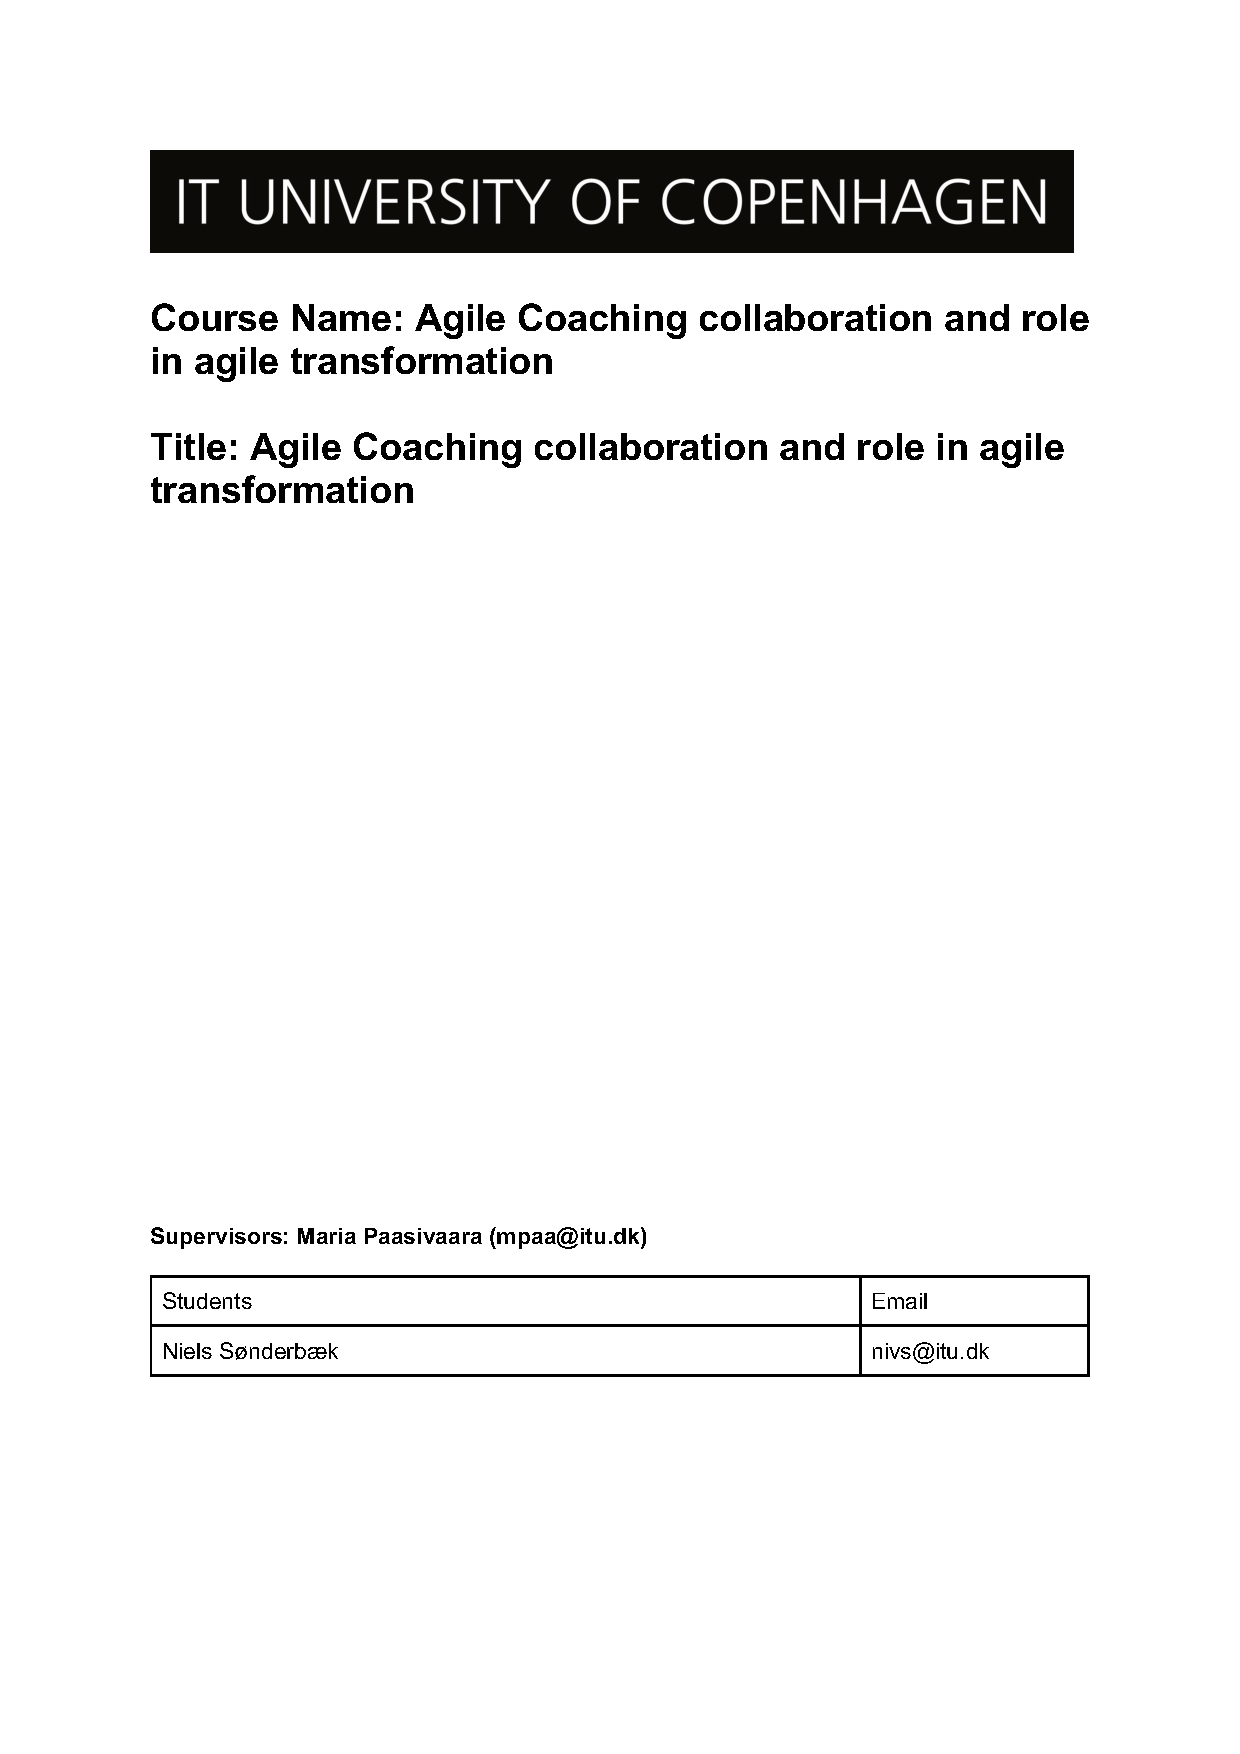
\includegraphics[scale=0.99]{frontpage.pdf}

\newpage

\restoregeometry

\section*{Abstract}
There is a trend for large-scale non-agile organizations to transition to agile to gain the benefits of this methodology. A new role has emerged as these organizations gradually or completely transition to agile, namely agile coach. In this study, the agile coach responsibilities, collaboration and the challenges of agile coaches are studied in the context of a large-scale agile transition. The study is based on a qualitative single case study. 
The agile coach responsibilities were found to be \emph{onboarding the organization to agile, ensure agile ways of working, build trust, build leadership relationship, ensure cross tribe collaboration and others}. The agile coaches were found to collaborate with other agile coaches on subjects and challenges related to their daily work, collaborate with product owners on impediments the product owner or the team would have and collaborate with tribe leads on ensuring that agile initiatives were prioritized and completed. Lastly, agile coaches experienced challenges such as being too few to effectively carry out their responsibilities, having to coaching remotely due to Covid-19, changing a deep top-down management culture, a lack of focus on agile and having to transition a sales department to agile.
The findings are mainly in-line with existing findings of the agile coach responsibilities and challenges. The agile coaches were found to mainly collaborate with Product owners, Tribe leads and other agile coaches. The structure of the collaboration between agile coaches contained new discoveries for this craft.

\newpage
\section*{Acknowledgements}
I would like to thank my supervisor Maria Paasivaara for her time, her guidance and invaluable feedback doing this project. I would like to thank Jesus Lopez de Paz at Nuuday for allowing me to study his agile coaches and for giving me a forum to recruit participants. I would like to thank Henrik Harder at Nuuday for allowing me to take time off to complete this thesis. I want to express my gratitude to all the individuals, who allowed me to interview them and gain insights into the roles on which this thesis is build.
\newline
\newline
\noindent I also wish to thank all dear to me, who supported me through this entire education and especially doing the last month of completing this thesis. Without you, this thesis would not exist and I am forever grateful to you.

\newpage

\tableofcontents

\newpage

\chapter{Introduction}
This chapter provides an introduction into the motivation for this thesis, what the background of it is, an overview of the Spotify model, the authors relationship to the case company and what research problem and question are addressed.

\section{Motivation}
The benefits of agile methods has made them attractive for larger companies to adopt. There is an industry trend to adopt agile methods at a large scale \cite{dikert2016challenges}. However, little research literature exists for large-scale agile transformations \cite{paasivaara2018large}. One of the factors to a successful transformation, which has been identified in the existing literature is coaching \cite{dikert2016challenges} \cite{paasivaara2018large} \cite{uludag2018identifying}. A way to achieve coaching in a organization is to utilize the agile coach role. The agile coach role has been studied by several researchers \cite{litReviewACRole} \cite{althoff2019qualitative} \cite{stray2020agile} \cite{parizi2014hidden}, but little research exists on the agile coach role and collaboration during a large scale agile transformation. As there seems to be an increasing trend towards large scale agile transformations and that agile coaches have been identified as one of the factors to a successful transformation additional research into the role would further the understanding on how to conduct such a transformation successfully.

\section{Case background}
TDC Group is a Danish telecommunication company, which has operated in more than 140 years nationally \cite{tdcHistory}. Their mission is to \textit{build and support an innovative, open model that will ensure all of Denmark connects to the new digital opportunities} \cite{tdcHistory}. The organization employees 7000 people, has more than 6 million customers and a revenue of 17 billion DKK with an EBITDA of 6.5 billion DKK \cite{tdcGroupAnnualReport}. TDC group had been experimenting with agile methods for a few years through out the company prior to the separation \cite{HenrikNuudayPresentation}. They had been using the Spotify model, which is a method invented at Spotify for scaling Agile at a large scale and across several teams  \cite{spotifyMethod}. A detailed explanation of this model will be given in \autoref{spotifyModelBackgroundInfo}.

In 2018, TDC group announced that they would be changing the structure of their organization, creating two separate business units, known as Opco and Netco at the time \cite{tdcSplitAnnouncement}. In 2019, Opco got rebranded to Nuuday and was legally separated from Netco \cite{tdcNuuday}. Nuuday consists of 9 individual brands such as YouSee, Telmore, TDC Erhverv etc \cite{nuuday}, they employ 4515 people \cite{tdcGroupAnnualReport} and has a revenue of 15,626 billion DKK with an EBITDA of 1,964 billion DKK \cite{tdcGroupAnnualReport}. In the fall of 2019, Nuuday announced that they would undergo an Enterprise agile transformation on April 1, 2020 \cite{acTeleEnterpriseAgileNuuday}, which would entail using agile methods for large parts of their organization. The transformation would be rolled out all at once on April 1st except for a few support departments \cite{HenrikNuudayPresentation}. Nuuday decided to hire 40 additional agile coaches to assist with the transformation and support the organization in the new structure and agile methods \cite{HenrikNuudayPresentation}. On May 1, 2020 Nuuday went live with their Enterprise Agile transformation, adopting agile methods across the company and has been going through the transformation since.
A timeline of all the mentioned events can be found in \autoref{timelineApp}.

\section{Spotify model}
\label{spotifyModelBackgroundInfo}
The Spotifiy model was created to try to manage the challenge of scaling agile in a large-scale organization. The basis of the model is the organizational structure, which can be found in \autoref{spotifyModelVisualFig}. The organizational structure consists of squads, tribes, chapters and guilds. 

A squad is similar to a Scrum team, it is a collection of people sitting together in a cross functional team with end-to-end responsibilities \cite{spotifyMethod}. Each squad has their own long term mission such as onboarding customers or consuming content. There is no designated leader in a squad, but each squad does have a product owner. A product owner is a person, who is responsible for prioritizing the work, that is to be completed by the squad and to maintain a product backlog of work for the squad \cite{spotifyMethod}. Product owners collaborate across squads to maintain a high-level roadmap to show where the organization is headed at a high-level.

A tribe is a collection of squads, which work in related areas such as infrastructure, or streaming. Each tribe is lead by a tribe lead, who is responsible for providing the best environment for the squads which are part of the tribe. A tribe is co-located physically in the same office to promote collaboration between squads. The size of tribes are designed after the 'Dunbar Number', which says that people cannot maintain more than 150 social relationships with each other \cite{dunbar2010many}. Tribes should therefore be smaller than 150 people. Within the tribe, squads shows their work to each other through demonstrations and they learn from each other. 

A chapter is a collection of people that have similar skills and are working within the general same competency area \cite{spotifyMethod}. A chapter is constrained to be within a single tribe. Examples of chapters could be web development, backend development, product management etc. Chapters meet regularly to discuss their area of expertise and their challenges. A chapter is lead by a chapter lead, who acts as the line manager for the chapter members, dealing with the traditional responsibilities such a people development and salaries \cite{spotifyMethod}. A chapter lead is still part of a squad and is involved with day-to-day work to stay in touch with reality. 

A guild is a community of people that share knowledge, tools, code and practices within one interest. Guilds are not constrained by tribes. Each guild has a guild coordinator, who organizes and coordinate the corresponding guild. Examples of guilds are frontend guild, agile coaching guild, testing guild etc. Guilds are open to anybody, who has an interest for the subject of the guild.

\begin{figure}[!h]
    \centering
    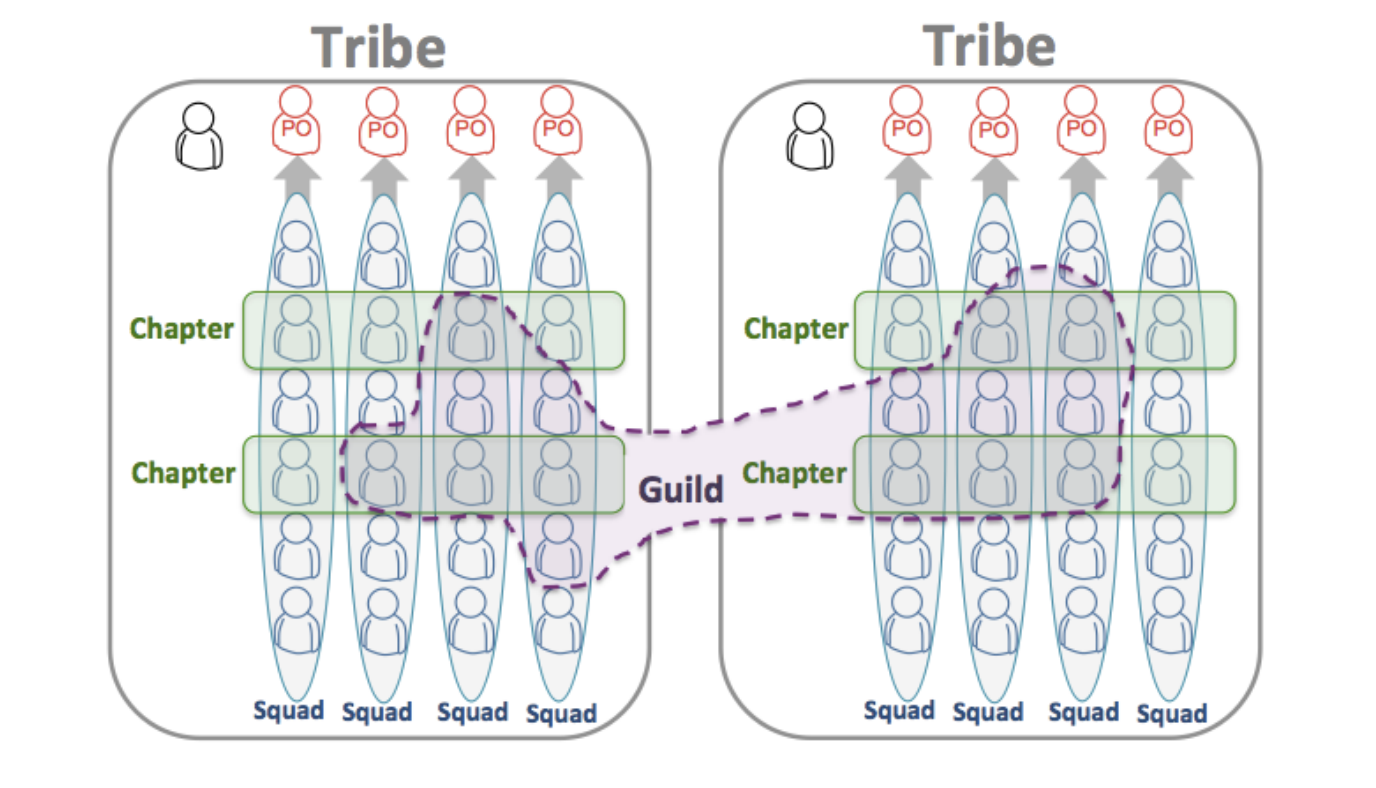
\includegraphics[scale=0.6]{SpotifyModelVisual.png}
    \caption{Illustration of Spotify model structure \cite{spotifyMethod}}
    \label{spotifyModelVisualFig}
\end{figure}

\section{Author relationship to company}
The author was part of one of the experiments using agile methods in TDC Erhverv while undertaking a master degree in Computer Science at ITU. During the time in TDC Erhverv, the author got insights into how agile coaches operate and what some of their responsibilities are as a result of two agile coaches working in this department at the same time. The author was and still is employed by the case company and so when the transformation went live, the author had a first person insight into a large-scale agile transformations and some of the challenges associated with these on a practical level. At the time for beginning this thesis, the transformation had been going for 4 months and at that time there was now an option to interview a larger group of agile coaches, which had experience with the agile coach role in a large-scale agile transformation.

\section{Research problem and questions}
The aim of this research is to investigate the agile coach role in large-scale agile transformation and how the agile coaches collaborate among themselves and other roles. To achieve this, the author poses the following research questions:
\newline

\textbf{RQ1:} \emph{What is the responsibility of an agile coach in a large-scale transformation?}

\textbf{RQ2:} \emph{Who does agile coaches collaborate with?}

\textbf{RQ3:} \emph{What does agile coaches collaborate about?}

\textbf{RQ4:} \emph{What are the challenges of being an agile coach?}

\chapter{Related work}
In the following chapter, the existing literature of the subject will presented. The knowledge about large-scale agile transformation, the associated challenges and success factors to this kind of transformation  will be laid out in \autoref{largeScaleAgileTransformationRelatedWork}. The literature about the agile coach role and skills will be presented in \autoref{agileCoachRelatedWork}.

\section{Large scale agile transformation}
\label{largeScaleAgileTransformationRelatedWork}
The requirement for a transformation to be 'large scale' is not exact and as discussed by Dikert et. al \cite{dikert2016challenges} different research publications and conference workshops denotes different requirements such as number of people involved, amount of teams, certain project cost and size of codebase. For this research, the definition of large scale will follow \cite{dikert2016challenges}, following thereby that {\textit{
software development organizations with 50 or more people or at least six teams}}.
The transformation to agile at a large scale can be performed either as a big bang approach or gradually. With the big bang approach, the entire organization is transformed at one point and will adopt agile methods from one day to another. Such an approach was seen at Salesforce, where they completed a big bang transformation of a 200 person team \cite{fry2007large}. Fry \cite{fry2007large} does mention, that while existing literature does suggest to make an gradual transformation, Salesforce chose to do a big bang transformation to \textit{avoid organizational
dissonance and a desire for decisive action. Everyone would be doing the same thing at the same time}. Salesforce has previously implemented agile methods in one team successfully prior to the big bang transformation. 
In contract to big bang, gradual transformation typically begins with one or more experiments with agile methods \cite{gandomani2013exploring} \cite{benefield2008rolling} \cite{goodman2008s} often referred to as pilot projects in which it is possible to evaluate the agile methods within the organization and fine tune what suits the organization in regard to agile.

\subsection{Challenges of large scale agile transformations}
Agile methods are meant to be used in small and stand alone projects \cite{boehm2005management}. Therefore, it must be expected that certain challenges will arise when trying to scale the usage of agile methods across several teams and projects. Dikert et al. has performed a systematic literature review of the challenges with large scale agile transitions \cite{dikert2016challenges}. The challenges which is related are related to the agile coach role and responsibilities will be outlined in \autoref{LargeScaleAgileChallenges}.

\clearpage
\begin{table}[!ht]
\begin{tabular}{|p{5cm}|p{8cm}|p{1cm}|}
\hline
\textbf{Challenges} & \textbf{Description} & \textbf{Source} \\ \hline
Change resistance   & People will resist to change, if they do not understand the reason(s) to change and the change is perceived as hard. It should not be expected that everyone is willing to accept the change and some people will resist the change for all time. People can be skeptic towards the new way of working. Having the change mandated top-down will effect negatively, if the change is presented badly. If managers doesn't accept and support the change, they have the option to undermine the entire change.   &    \cite{dikert2016challenges}     \\\hline
Lack of training and coaching & A lack of training will leave people unprepared for the change and can lead to lower motivation. A lack of coaching in the new way of working in real settings would effect the necessary mindset change. Demand for coaching often exceed supply of available coaches and in certain cases less seasoned people was appointed as agile coaches.   &    \cite{dikert2016challenges}     \\\hline
Organizational boundaries & Internal silos can exists within the organization, which can cause issues with the agile implementation. Different teams can come to operate with different prioritizes and agendas.   & \cite{dikert2016challenges} \\ \hline
Too high workload & The workload is not adjusted to encompass the current state of transformation and in some cases overloaded people will not be able to change to the new ways of working and culture.  &    \cite{dikert2016challenges}     \\\hline
Integrating non-development functions   & Non-development roles can resist the change and for the transformation to be successful, the entire organization must embrace the new way of working. &    \cite{dikert2016challenges}     \\\hline
\end{tabular}
\caption{Large scale agile challenges}
\label{LargeScaleAgileChallenges}
\end{table}

\clearpage

\subsection{Success factors of large-scale agile transformations}
In contrast to the challenges of a large-scale agile transformation, several success factors have also been identified. While identifying the challenges of large-scale agile transformations, Dikert et al. \cite{dikert2016challenges} also reported the found success factors for such a transformation. In \autoref{LargeScaleAgileSuccessFactors} the relevant findings to the agile coach role and responsibilities have been listed and explained.

\begin{table}[!ht]
\begin{tabular}{|p{4cm}|p{8cm}|p{1cm}|}
\hline
\textbf{Success factor} & \textbf{Description} & \textbf{Source} \\ \hline
Management support   & Management must support the change sincerely as they have the authority to remove impediments and insist on working with agile. Management also allocates time and resources for training and coaching, which is another success criteria. A proper education of agile to management is also important to gain support.  &    \cite{dikert2016challenges}     \\\hline
Training  & Agile training will improve the change of a successful transformation and in some cases it was reported that the transformation would fail without proper training. Training can lead people to be more inclined towards transformation and even enthusiastic about it.   &    \cite{dikert2016challenges}     \\\hline
Coaching   & Agile practices are best learned by doing and coaching teams while they were using agile methods in practice is an important factor. Without coaching, teams can apply incorrect agile practices and damage the transformation. Other benefits of coaching are watching and correcting issues as they arise, draw attention towards understanding the principles of agile. Both internal and external coaches are beneficial as they provide different perspectives.  &   \cite{dikert2016challenges}     \\\hline
\end{tabular}
\caption{Large scale agile success factors - part 1 of 2}
\label{LargeScaleAgileSuccessFactors}
\end{table}

\begin{table}[!ht]
\begin{tabular}{|p{4cm}|p{8cm}|p{1cm}|}
\hline
\textbf{Success factor} & \textbf{Description} & \textbf{Source} \\ \hline
Mindset and Alignment   &  The principles of agile should be emphasized over practices and simple mechanics as it will provide an understanding of the value of the change. Social events were shown to benefit building an agile mindset. The organization must be aligned towards a common goal of the new ways of working. &    \cite{dikert2016challenges}     \\\hline
Team autonomy   &  Teams needs to have the autonomy to self organize and implement the agile methods fitting to their team. This will create commitment and motivation to continue using agile and improve it.  &    \cite{dikert2016challenges}     \\\hline
Requirements management   & The Product Owner role can attribute to making the team perform better and ensure that the product is implemented correctly if the role is implemented correctly and the Product Owner is performing well. The Product Owner should receive training and coaching in agile methods and in particular to agile methods attaining to their role.  &    \cite{dikert2016challenges}     \\\hline
\end{tabular}
\caption{Large scale agile success factors - part 2 of 2}
\label{LargeScaleAgileSuccessFactors2}
\end{table}

\clearpage

\section{Agile coaching}
\label{agileCoachRelatedWork}
The responsibilities of an agile coach are to coach and facilitate agile teams and managers in both adapting and implementing agile practices, processes and other values found in software development \cite{parizi2014hidden}. The role has emerged as organization transition gradually or completely to agile and coaching has been identified as one of the key factors for a successful transition to agile \cite{dikert2016challenges}. Adopting agile is not trivial as several challenges such as resistance to change, lack of customer collaboration and lack of experience of knowledge of agile methods and practices stand in the way of the adoption \cite{dikert2016challenges} \cite{litReviewACRole}. 
There exists several practitioner’s guides and books on agile coaching and the role of an agile coach \cite{davies2009agile} \cite{belling2020agile}. Certifications for the role are available through several providers \cite{icaACCertification} \cite{scrumAllianceACCertification}. In academic research literature some studies exist on how agile coaches practice agility at companies and through agile transitions \cite{hanly2006agile} \cite{silva2007growth} \cite{backlander2019doing}. 

\subsection{Agile coach role}
Stray et al. \cite{litReviewACRole} have performed a systematic literature review of agile coaching and the agile coach role. In the following paragraphs their findings relevant to the responsibility and collaboration of an agile coach will be outlined.
\newline
\newline
\noindent\textbf{Build and training of teams} \newline
The primary role of agile coaches was found to be building teams by providing support in their implementation of agile methods and training the team to be become self-organized. The coaches also teach agile techniques and tools and conduct workshops and training in agile methods.
\newline
\newline
\noindent\textbf{Enlighten stakeholders and management on agile methods}\newline
An agile coaches responsibilities are not limited to individual teams. Their stakeholders are all parties, which are part of the agile transition process. The coach must coach all the stakeholders in their role and responsibilities. In particular, agile coaches must support Scrum Master and Product Owners. The coaches are typically organized such that they are within a team, while working with several teams and also support the entire organization with other coaches and leaders. 
\newline
\newline
\noindent\textbf{Facilitate and monitor the implementation of agile}\newline
The agile coach will facilitate and monitor implementations of Scrum practices, collaborate on potential issues, suggestions and innovations and provide solutions for teams to take more ownership for the actions. The facilitation is carried out by proposing required adjustments in the adoption of agile methods and practices. Furthermore, they assist the stakeholders in solving their challenges during the transitions and they facilitate the change process.
\newline
\newline
\noindent\textbf{Customize agile methods to the context of their respective projects}\newline
For a successful agile adoption, the methods and processes must be customized to the context of their respective projects. Therefore, the agile coach must understand the respective context such that they can adopt the fitting methods and processes for that particular project.
\newline
\newline
\noindent\textbf{Assist with guidelines, setting goals and roadmaps}\newline
Agile coaches collaborate with management to define common goals for the organization, creating a roadmap of the future of the organization and how they will achieve these goals. Agendas and instructions for teams are also created and guidelines for the full agile transformation.
\newline
\newline
\noindent\textbf{Build trust}\newline
To build trust with the teams they coach they must utilize frequent and open communication. 
\newline
\newline
\noindent\textbf{Remove bottlenecks for successful teamwork}\newline
A focus of an agile coach is to assist the team in being productive and successful. When a bottleneck to being productive or successful is encountered in a team, the agile coach will try to remove the bottleneck in the appropriate manner.

\subsection{Agile coach skills}
In the research by Stray et al. \cite{litReviewACRole}, they also examined what skills was required for an agile coach. Four main types of skills was found, which are presented below.
\newpage
\noindent\textbf{Leadership skills} \newline
Leaderships skills and qualities are the most important set of skills, which an agile coach must posses. Leadership skills such being able to communicate well, understand teamwork and team dynamics, team building and conflict management. Furthermore, a coach need to be able facilitate learning, which requires strong social skills. Traits such as positivity, persistence and patience will support the above mentioned leadership skills and qualities.
\newline
\newline
\noindent\textbf{Project management skills} \newline
With proper project management skills, agile coaches are able to achieve goals and meet success criteria at certain times including change management, system risk management, knowledge management skills and enabling teams to make more realistic estimates
\newline
\newline
\noindent\textbf{Expertise in agile methods and practices} \newline
Given that the agile coach must train and coach in agile methods and practices, the knowledge of such is a necessary skill. As mentioned previously, there does exists certifications for agile coaches, but the necessity of such is debated.
\newline
\newline
\noindent\textbf{Technical skills} \newline
As an agile coach often translates between business terminology and technical language used by teams or may question a proposed technical solution, they need technical skills such as diversity in IT skills together with software design and development skills.

\subsection{External vs internal agile coach}
Organizations can utilize external coaches and/or internal coaches when transitioning to agile. In some organization, external coaches are brought in for the initial training and startup \cite{litReviewACRole}. The external coaches can help train internal coaches, who will take over the coaching responsibilities at a later stage \cite{litReviewACRole}. External agile coaches can provide an impartial view on the company and diverse experience, whereas internal coaches understands the context of the company’s business and processes \cite{o2014assessing}. 
There are several examples of organizations, which have utilized external agile coaches \cite{hanly2006agile} \cite{fry2007large} \cite{benefield2008rolling}. In these cases, the demand for agile coaches were so large, that external agile coaches had to be brought in or the external coaches provided the foundation to build the agile transformation upon. 
However, Parizi et al. \cite{parizi2014hidden} recommends to hire on-site agile coach full time rather than external as teams will face different challenges at various times and therefore need the support of a full time coach. This can further be supported by the fact that the benefits of having an agile coach employed have been found to outweigh the cost \cite{o2014assessing}.

\chapter{Research Methodology}
\section{Approach}
This study is based on a qualitative single case study. This approach has been chosen as the agile coach role in large scale transformations and their collaboration is not thoroughly researched in practice\cite{litReviewACRole}.
\section{Problem and questions}
As mentioned earlier, the aim with this study is to investigate the agile coach role in large-scale agile transformation and how the agile coaches collaborate among themselves and other roles. This aim gives to the following research questions:
\newline

\textbf{RQ1:} \emph{What is the responsibility of an agile coach in a large-scale transformation?}

\textbf{RQ2:} \emph{Who does agile coaches collaborate with?}

\textbf{RQ3:} \emph{What does agile coaches collaborate about?}

\textbf{RQ4:} \emph{What are the challenges of being an agile coach?}

\section{Case selection}
Nuuday went live with their large-scale agile transformation, referred to as 'Enterprise Agile' on May 1st, 2020 \cite{HenrikNuudayPresentation}. During this transformation, 24 new tribes and 200 new squads would be created, meaning that most of the organization would be restructured and all tribes and squads would utilize agile to function. Prior to the transformation, several pilots had been conducted around the organization and several agile coaches were already employed with the company \cite{HenrikNuudayPresentation}. During December 2019 till February 2020, 40 new agile coaches were employed. This research was carried out during the fall of 2020, therefore data from both prior the transformation, during the transformation and future predictions regarding the agile coach role and the transformation could be obtained.\newline
The author was employed at the case company before the transformation and was employed at the company at the time of this thesis, which is 8 months after the transformation went live. Therefore, the author has access to the agile coaches at the case company and was able to interview a larger subset of the coaches, that was has previously been done \cite{althoff2019qualitative}. 
\section{Data collection}
% Why this sample, why different coaches and roles and experience?
To collect relevant data about the research problems, semi-structure interviews were conducted with 15 agile coaches including 3 agile coach chapter leads. The interviewees were selected based on volunteering while also attempting to get a variety of experienced coaches, new coaches and chapter leads. The interviews were mainly conducted online with the case company chosen communication tool as the research was carried out while Covid-19 was still an issue during the data collection phase and the case company advised to generally hold all meetings online during this time. Video and sound were available during the online interviews, however only audio was captured as agreed upon by the interviewees. The interviews lasted between 30-60 minutes. The interviewee role, interview type and length of interview details for each interview can be found in \autoref{Interview overview}. 
The type of interview was divided into two; one for agile coaches and one for chapter lead agile coaches. Several questions were the same, while some was tailored for the specific role. The interview templates can be found in \autoref{Interview templates}. During the first interview with an agile coach, knowledge about a recent reorganization of their respective tribe was shared and subsequently two questions was added to the interview template for agile coach chapter leads (question 15+16 \autoref{acCLInterviewTemplate}).
\section{Data analysis}
The interviews were transcribed using transcribe by wrelly \cite{wreallyTranscribe} and every transcription was reviewed and corrected by the author. The transcripts was transferred to ATLAS.it \cite{atlastCodingSoftware}, where an inductive coding process was performed stemming from the research questions. Background information was likewise noted during the coding process for documentation and general notes to help explain some of the answers was taken. The most used codes was: 
\begin{itemize}
    \item Collaboration
    \item Remote coaching
    \item Responsibility 
    \item Transformation responsibility
    \item Agile maturity
    \item Challenges
\end{itemize}
\section{Data validation}
The participants in this study was selected from different roles and backgrounds to ensure variety in the sample size. The results from this case study were presented to the participants in a joint session, where the participants could invalidate or validate the results. One of the results was not recognized by one of the participants, but it was recognized by two others and this particular result has been noted such that it doesn't reflect that this is a result that is applicable to all the agile coach participants. 

\chapter{Results}
\label{results}

In the following section, the results from the interviews will be presented. In \autoref{AC background} the background for the agile coaches will be presented. In \autoref{AC responsibility} the different responsibilities will be presented including agile methods, culture and mindset both prior, during and after the transformation. The different collaboration between agile coaches, product owners and tribe leads will be presented in \autoref{Collaboration}. Remote coaching, coaching prioritization, agile sales and other challenges will be presented in \autoref{Challenges}.

\section{Agile coach background}
\label{AC background}
In the months leading up to the transformation 40 additional agile coaches were hired. All the interviewed agile coaches were hired internally. Prior to being agile coaches, 13 out of 15 of the agile coaches already had several (2+) years of experience with agile and using it intentionally. The other two coaches were following the principles of agile \cite{agileManifesto} in their ways of working, but did not use specific agile methods such as Scrum, Kanban or SAFE. Two of the coaches have a large degree of domain knowledge in the current industry of Telco's and was employed for several years in the case company prior to becoming agile coaches.

\noindent Five of the coaches had previously been scrum master at the case company and several saw being an agile coach as either an extension of a scrum master or the natural next step.

\begin{displayquote}
\textit{
...if you are a scrum master, I believe that there's a point in your career where it's very natural to start something else... so, yeah for me, it was a natural progression either you become an agile coach, you become, you switch company and try something else... - AC 7
}
\end{displayquote}

\noindent The agile coaches were hired in two batches, where 9 coaches were hired in batch 1 and 6 coaches were hired in batch 2 of the study participants. The coaches in batch 1 had two more months of onboarding time, where they had the opportunity to shadow existing agile coaches together with pre-transformation squads and gain practical experience in these squads together with the existing agile coaches. The second of batch of agile coaches were hired in February after an internal hiring, that was open to all employees.  

\begin{displayquote}
\textit{
Not only reading about, but try them out in practice. I was so lucky that I got a squad in [redacted] to follow and to ask stupid questions and try exercises on stuff like that. - AC 5
}
\end{displayquote}
\begin{displayquote}
\textit{
...and the last thing was obtaining practical knowledge trying out something in practice... we had the opportunity to actually go observe previous agile coaches in their ways of working and actually having squads in another tribe... I went out and facilitate and coach them in some way of working in agile... - AC 7
}
\end{displayquote}
The overview of the different backgrounds for agile coaches can be found in \autoref{AC background table}.

\newgeometry{left=0.75in}
\begin{table}[!ht]
\begin{tabular}{|p{1.5cm}|p{3cm}|p{3cm}|p{2cm}|p{2.3cm}|c|c|}
\hline
\textbf{Coach\#}  & \textbf{Several years} of \textbf{agile experience} & \textbf{No formal agile experience} & \textbf{Agile coach} & \textbf{Scrum Master} & \textbf{Batch 1} & \textbf{Batch 2} \\ \hline
\centering\#1   &                            &    \centering      X                &             &     & \centering X &         \\\hline
\centering\#2   &       \centering X                    &                           &             &     && X        \\ \hline
\centering\#3   &       \centering  X                   &                           &    \centering  X       &    \centering  X     & \centering X &   \\\hline
\centering\#4   &       \centering    X                 &                           &             &   &&  X        \\\hline
\centering\#5   &     \centering       X                &                           &             &       &X&       \\\hline
\centering\#6   &     \centering        X               &                           &             &      \centering X  &&  X    \\\hline
\centering\#7   &     \centering       X                &                           &             &    \centering   X  &  X &     \\\hline
\centering\#8   &     \centering       X                &                           &             &     \centering  X   &&  X    \\\hline
\centering\#9   &      \centering      X                &                           &    \centering  X       &       & \centering X &       \\\hline
\centering\#10   &     \centering      X                 &                           &    \centering  X       &      & \centering X &        \\\hline
\centering\#11   &     \centering      X                 &                           &   \centering   X       &      & \centering X &        \\\hline
\centering\#12   &                            &        \centering     X              &             &      & \centering X &        \\\hline
\centering\#13   &     \centering       X                &                           &             &      && X        \\\hline
\centering\#14   &     \centering     X                  &                           &   \centering  X        &     &X&         \\\hline
\centering\#15   &    \centering       X                 &                           &             &      \centering  X    && X  \\\hline
\textbf{Total} &      \centering      \textbf{13}                &       \centering    \textbf{2}                &  \centering  \textbf{5}         &  \centering   \textbf{5} & \centering \textbf{9} & \textbf{6} \\\hline   
\end{tabular}
\caption{Agile experience, has been Scrum master or Agile coach previously overview for all interviewees}
\label{AC background table}
\end{table}
\restoregeometry

\section{Agile coach responsibility}
\label{AC responsibility}
In this section, the following research question will be answered:
\newline

\textbf{RQ1:} \emph{What is the responsibility of an agile coach in a large-scale transformation?}
\newline

\noindent The agile coach responsibilities found in this study can be found in \autoref{AC responsiblities table}. The agile coaches responsibilities changes based on what stage of the transformation they are in. Therefore, the responsibilities have been grouped by transformation stage and a more thorough explanation of the responsibilities will be given in the following sub sections.

\begin{table}[!ht]
    \centering
    \begin{tabular}{|l|p{2.7cm}|p{2.7cm}|c|} \hline
      \textbf{Responsibilities} & \makecell{\textbf{Prior to} \\ \textbf{transformation}}  & \makecell{ \textbf{During} \\ \textbf{transformation}  }  & \textbf{Next stage} \\ \hline
       Learning the craft & \centering X &  &  \\ \hline
       Produce agile material & \centering X &  &  \\ \hline
       Prepare for onboarding & \centering X &  &  \\ \hline
       Onboarding organization to agile &  & \centering X &  \\ \hline
       Ensure agile ways of work &  & \centering X &  \\ \hline
       Teach agile roles &  & \centering X &  \\ \hline
       Build trust &  & \centering X &  \\ \hline
       Build leadership relationship &  & \centering X &  \\ \hline
       Ensure cross tribe collaboration &  &  & X \\ \hline
       Higher strategic focus &  &  & X \\ \hline
    \end{tabular}
    \caption{Agile coach responsibilities prior, during and in the next stage of the transformation}
    \label{AC responsiblities table}
\end{table}

\subsection{Responsibilities prior to transformation}
Prior to the transformation entails the time the agile coach was hired, which was in December 2019 or February 2020 respectively five or three months before the transformation went live. Of the interviewed coaches, there was six coaches, who had not either been a scrum master or an agile coach prior to the transformation. Ten of the coaches was not an agile coach prior to the transformation. Therefore, one of the major responsibilities for these coaches was learning the craftsmanship of being an agile coach in theory such as teamwork, product management, facilitation, educating etc. The coaches received training from an external partner and from workshops put together by the agile coach chapter leads. Each coach was assigned to a study group and groups presented different topics for all the agile coaches.

\begin{displayquote}
\textit{
...in that time frame my main responsibility was to focus on my own Learning Journey to become good at my new craft, which I had a little experience with but not a lot but to get to know what tools I should put in my toolbox and have some sort of idea of how I can use those tools out in the real world. - AC 5
}
\end{displayquote}

\begin{displayquote}
\textit{
And then I was doing I was one of the guys who had experience as a Scrum Master not that much, but but more than most so I also did a lot sparing with my colleagues, agile coach colleagues I pretty much attended everything I could regarding this transformation. - AC 6
}
\end{displayquote}

\noindent The coaches from batch 1 had the opportunity to also gain practical experience by shadowing existing agile coaches in their work. That followed that some of the existing agile coaches were asked to maintain their coaching job such that shadowing was possible. 

\begin{displayquote}
\textit{
I still had a team, it took me a while to let go of the team because what we were told was, we were told in the beginning to maintain our old roles us that were coaches because then we could have the new ones come and follow along. - AC 3 
}
\end{displayquote}

\begin{displayquote}
\textit{
I stayed on as an agile coach while doing all the other stuff and also had some new agile coach is shadowing me in that period. - AC 11
}
\end{displayquote}

\subsection{Responsibilities during the transformation}
The responsibilities covers the time frame when the case company went live with the transformation May 1st 2020 and until the coach was interviewed, which was in October 2020. Almost the entire organization had be restructured and much of the organization had never worked agile before, so the agile coaches facilitated a bootcamp, where the new teams could meet and organize themselves while also learning how they should work agile in these new teams known as squads. The bootcamp lasted 1 day and was held physically onsite, but with some of the participants participating remotely because of Covid-19. 

\begin{displayquote}
\textit{
I think we had like we had the first day of bootcamp, right and the boot camp was luckily for us mainly on site because we were such a small department which was great in that case a so you can actually meet everyone for the first time, see how they are. - AC 13
}
\end{displayquote}

\noindent After After the bootcamp, the agile coaches started focusing on the squads and teaching them about the ceremonies, which was applicable to the agile framework, that the squad had chosen to use. They also spend time on teaching what new roles entailed and did not entailed such as product owner, chapter lead and leadership. 

\begin{displayquote}
\textit{
In the very beginning, we had some sessions and some general learning sessions with the POs and the chapter leads and Leadership, where we trained them in some basic principle
} - AC 3
\end{displayquote}

\noindent Some coaches reported that they spend some time to build trust and a healthy work environment in this stage of the transformation. They build trust both in the squads and towards themselves such that they could be more effective in their coaching. 

\begin{displayquote}
\textit{
...figure out getting to know people because that's that's the first step really you cannot really coach anybody if you don't have a trust relationship between you so that was our main focus, my main focus to begin with getting to know people and just basically to talk to people. - AC 5
}
\end{displayquote}

\noindent The relationship between the tribe lead and the agile coach was also reported as focus for most agile coaches. They sough to build trust with the tribe lead, have regular interaction with him or her and align both their agile vision and the tribe lead's vision. Some of the tribe leads had never worked with agile before, so they relied and trust the agile coaches to handle that within the tribe. Some of the coaches have been a right hand man/woman to the tribe leads and could be a sounding board as the agile coaches were close to the squads on a daily basis.

\begin{displayquote}
\textit{
we doing more sparing with the with the tribe lead lot of sparing with the tribe lead coordination with him making sure that that he has the right mindset making sure that that we are aligned with our work with what he wants to do is his tribe, so that's I'll say 50\% of my time. - AC 4
}
\end{displayquote}

\begin{displayquote}
\textit{
I become a an important figure for my tribe lead because I am with the squads on a day-to-day basis. I hear what they say and I can translate it into a bigger picture without being kind of a liar, but I have a cool tribe lead really just wants to make cool place to be so yeah kind of changing, you know leadership in a good direction and that I think is also very important for an agile coach. - AC 7
}
\end{displayquote}

\subsection{Responsibilities in the next stage of the transformation}
When asked when the transformation will end, almost all coaches had the same response: "never" and most preferred to rather use the word 'journey' rather than transformation and therefore the responsibilities in this section includes what responsibilities the agile coaches expected to be performing in the next stage of the agile journey. 
The next step for the coaches to tackle is cross tribe collaboration, which currently is happening through an Objectives and Key Results (OKR) process \cite{wodtke2016introduction} performed every quarter. The current process is not thought off as ideal and can be improved upon.

\begin{displayquote}
\textit{
we are all focused on our own tribe, you know, just making the tribe work. Making the squad's work is even not even tribes making the squads work is the first step. They're making the tribe then I think we have to think cross tribe somewhere in this in a year's time or maximum two years time. We will have to go there. - AC 8
}
\end{displayquote}

\noindent The agile coaches are currently placed under strategy in the organization structure and they do collaborate with strategy on several initiatives such as the OKR process. In the future, strategy will become an even bigger part of the agile coach responsibility as agile was also seen as a strategic goal. 

\begin{displayquote}
\textit{
Well, I hope will end up being more strategic level. Where we are is not much focusing on tools as much as we are focusing now... we as coaches have more free time to focus at the tribe lead and also in the other tribes how can we work better and how can we set strategies, how can we define that for the future? - AC 15
}
\end{displayquote}

\noindent When we attempt to predict the future, a difference in response is to be expected and some of the responses of the agile coaches would contraction each other. They believed that they will be have more high level responsibility and become a flow to work resource, meaning that they would be staffed with different full-time tasks based on need \cite{flowToWorkDefinition}. Others believed that they would be more inclined to take over the scrum master role full time.

\begin{displayquote}
\textit{
 I think my role will change I would be more like a flow to work agile coach. The squad will not be so dependent on me. And I can come in and help them fine tune how they for them to be more efficient not effective efficient. - AC 2
}
\end{displayquote}

\begin{displayquote}
\textit{
 I think that we will have a hat in the future and the near future called scrum master just like we have the hat of PO and we will work much more closely with these people - AC 6
}
\end{displayquote}

\section{Collaboration}
\label{Collaboration}
In the following sections, the findings for who the agile coaches collaborate with, how they collaborate among themselves and other roles and what their views on the importance collaboration will be laid out. These the findings will be answering research question 3 and 4.
\newline
\newline
\indent \textbf{RQ2:} \emph{Who does agile coaches collaborate with?} \newline
\indent \textbf{RQ3:} \emph{What does agile coaches collaborate about?}
\newline

\subsection{Agile coach to agile coach}
\noindent At the case company, the agile coaches operate as a separate unit in their own tribe and they are distributed through out the organization. In some cases, several agile coaches are associated with assisting one tribe and in other cases a single agile coach is assisting an entire tribe by themselves. This entails that some agile coaches have the options to form partnerships with their co-coaches in the same tribe, which some has taken advantage of and has formed close collaboration with their co-coach(es). Informal daily check-ins has been established, where the coaches coordinate where they are at and what they are working on. These check-ins usually last about 15-30 minutes depending on what subjects needs to be discussed.
The coaches, who does not have a co-coaches has established partnerships with other agile coaches in related tribes in which they get to know each other tribes, discuss what each coach is dealing with currently and spare with each other. 

All the agile coaches belong to a chapter, however it was mixed if the chapter was used for collaboration. In the case where the chapter was used for collaboration, the agile coaches in the chapter had non-mandatory daily check-ins of 30 min length, where the participants could share what they were working on, get feedback or discuss something in regard to their specific tribe. The coaches in this kind of chapter would try to at least participate a few time weekly, depending on how busy they were. 

As mentioned, the agile coaches operate as their own tribe and they have a tribe weekly meeting, which they have named show-and-tell. On these meetings, the agile coaches will receive important information, coaches will show what they are working and it is an opportunity to get a feeling for where other other coaches are. This is the only formally agreed tribe wide collaboration event, which has been established.
Within the tribe, the coaches have established working groups to collaborate on a bigger subjects such as agile maturity assessment and OKR's, which pertains to the entire organization. These working groups are open to any agile coach, that wants to work on this subject and when the group have produced something, that needs to be shared with the rest of the coaches, it will be done so at a show-and-tell meeting. 

\begin{displayquote}
\textit{
So we kind have these working groups that sit down and really concentrate on one area that we have to do something about let's say we have to give all of PO's training in OKR's. Then we make some material for that in a smaller group. So that's one way of working with my colleagues. - AC 7
}
\end{displayquote}
 
\subsection{Agile coach to product owner}
For each tribe, there is a mandated product owner sync meeting occuring weekly or bi-weekly. The purpose of this meeting is for product owners to align the product vision across all squads, identify any cross squad dependencies and bring up any impediments they might have. The agile coaches participate in this meeting and they collaborate to help the product owners with both agile challenges, but also general team challenges which has been identified on the PO-sync or in other talks with the product owner. The product owners have become a collaboration partner as they are both the face of the squad and they are responsible for the future of their respective products. 

\begin{displayquote}
\textit{
I collaborate with PO's.. and I have bi-weekly check-ins with the POs of them just to see okay, what's going on? What do you need? What can we what can I do to help and that sometimes results in some workshops or something like all the activities like that? - AC 11
}
\end{displayquote}

\subsection{Agile coach to tribe lead}
Agile coaches work closely together with the tribe lead and have become the tribe leads trusted agile partner. Several of the coaches have arranged weekly meetings with the tribe lead, where they spare on what is going on in the individual squads as the agile coach are closer to the squads than the tribe lead and can validate if a challenge is something, that the tribe lead needs to deal with. The agile coaches utilize this relationship to further the agile agenda by providing feedback to the tribe lead on initiatives, which needs to be carried out such as doing agile maturity assessment, more workshops to teach agile methods or collaboration between squads. 

\begin{displayquote}
\textit{
Then I also have some one-on-one with my tribe lead of course. I have an hour a week or something like that. And it's actually quite fine, so we kind of spare on what's going on. What's happening in teams. What should he know about, that people haven't said and do I have however looked at some processes this really look stupid.... And I'm I have the liberty and the time so I can sit down and say what is the problem actually now I can go to him and say I know you've heard this before but I just have to tell you it is actually a problem and they actually need have some help so we're doing that - AC 6}
\end{displayquote}

\section{Challenges}
\label{Challenges}
In the following sections, the following research question will be answered:
\newline
\newline
\textbf{RQ4:} \emph{What are the challenges of being an agile coach?}

\subsection{Too few coaches}
At the time of the interviews, there was 46 agile coaches employed by the case company. It was mentioned that some of the agile coaches was on either maternity or paternity leave or on stress leave and therefore the amount of available agile coaches is less than 46. During a recent re-organization of the agile coach tribe, the agile coach chapter leads were also relived of squad responsibilities in other tribe, leaving even fewer coaches to coach the respective squads in the tribes. This amount of coaches is in comparison to 200 new squads, which were created when the transformation when live. Furthermore, there is no dedicated scrum master in the squads even if the team does utilize Scrum as their agile method. 
Most of the coaches believed that they were too few and more would be beneficial to carry out their role. Several believed that double the amount of coaches would be beneficial at the current stage of the agile journey. However, a worry about having more coaches was the future need for that amount of coaches and some coaches expressed concerns that it would then be to many coaches:

\begin{displayquote}
\textit{
No, we could we could be more as of now, but that would also mean that in yeah one year. We just have just had to let people go. - AC 12
}
\end{displayquote}

\begin{comment}
% Do I want this in or not?
\noindent During the recent re-organization of the agile coach tribe, a change was initiated where each agile coach now have the option to only focus on 3 squads at a time in the tribe they are coaching. 

\end{comment}

\subsection{Remote coaching}
The biggest challenge for the agile coaches was having to both onboard an entire organization to agile and practice agility remotely most of the time. As the organization made the transformation to agile, Covid-19 was still at a critical level in Denmark and therefore the agile coaches had to onboard the organization to agility with a 1-day bootcamp in individual squads rather than the planned several day bootcamp. The agile coaches were given the new bootcamp material 2 days in advance and the onboarding had to be carried out in a mix between in-person and remotely.

\begin{displayquote}
\textit{
I would reckon that. I mean we've really been hit by Corona. This is a lot of Corona stuff in this because we were supposed to have like a two-day onboarding bootcamp for the entire organization. That didn't happen. We had a boot camp. That lasted one maybe half a day or one day per squad and then the organization then I say the organization I say the leadership and HR expected. Now everybody's onboard it in the Agile way of working because they had four hours boot camp with an agile coach who had been given the material two days in advance. It's like okay is this what I'm supposed to be doing? - AC 1
}
\end{displayquote}

\noindent After the onboarding day, most of the organization stayed remotely for a while longer and the coaches had to carry out their work remotely. Several of the agile coaches expressed concerns about the lack of informal interactions. Such interactions as having a talk by the coffee machine or overhearing a conversation in which they would hear an issue and have the option to step in to help immediately. The agile coaches are co-located with the tribe, they are coaching, so that they were immediately available for the entire tribe, if necessary. Other than that, they had the chance to observe the squads in their daily work. They can ask to be invited to a squad meeting, if the squad is comfortable with it. Given that the agile coach is not part of any squad in their respective tribe either, they don't have any of the regular meetings to build trust between the tribe members and themselves. 

\begin{displayquote}
\textit{
I can see a big difference from sitting at home and to actually being on site with them every day. It makes a huge impact because it's just small things that you just don't write or call someone for but when you're there it's easier to just turn around and ask or you hear a dialogue between someone and you can jump in and help in that dialogue or explain something and you get to see how the team dynamics is with the team. You can't see that on the screen and if you're not even in their meetings, right, so it's a huge huge different to be on site. - AC 13
}
\end{displayquote}

\noindent The case organization allowed all employees to come onsite when Covid-19 was not as critical in the danish society, but as Covid-19 worsen during the fall of 2020 only 25\% of employees were allowed on-site at one time and so agile coaches had to chose which teams to be on-site with. Furthermore, they now had to solve more advanced challenges during this time without the option of explaining it in person or with their regular tools.

\begin{displayquote}
\textit{
Lockdown part two pretty difficult again, and I think I actually think it's more is both more stressful and more it's more difficult for me to handle because now we're not just talking cornerstones, right? We're not just telling them about so hey guys gather up. We need to talk about the PO role or we need to talk about some some ceremony. Now, we have trying to solve for some of the stuff that you know, it's just that much easier when you have a whiteboard or a pen or can look people directly in the eyes and just go back and forth or say Hey you have five minutes and it's really difficult to do that. - AC 12
}
\end{displayquote}

\subsection{Culture}
The case company has been part of an larger organization, which has existed for 138 years and therefore there is a deep culture of top-down management rooted by employees, that has stayed with the company for 25+ years \cite{tdcHistory}. Several of the existing employees has seen many transformations doing this time and have trouble trusting that the agile transformation will not be overtaken by another transformation soon. 

\begin{displayquote}
\textit{
...one of the things that happens when we do this, is that right now the organization saying ahh we're doing this agile thing and some people have been through, they have been at the company for 20-25 years and they have seen the last seven or eight transformations,  common goal "This Is The New Black". So I'm coming in and I'm saying I think we should do this in this and they are setting okay, but in three months time this will be over anyway, so why even bother? - AC 6
}
\end{displayquote}


\subsection{New craft}
Agile coaching is a craft and 8 of the 13 interviewed agile coaches had never been a coach before. So it was a challenge that they had to learn this new craft in a short time span, after which others considered them the experts of the craft. One of the challenges with this new craft was coaching rather than telling others what to do. Many of the coaches comes from roles, where they had mandate to either take their own decisions or have others carry out their decision. In the agile coach role they can only suggest and then the squads or individuals have to make a decision if they want to take the suggestion or carry on as previous.

\begin{displayquote}
\textit{
Well that it's a craftsmanship in itself right to do coaching and you can you can sometimes you can you can fall into some kind of pitfall and try to state your own opinion of some topic somehow somewhere. But but instead it you you should try to have it the ones that you are coaching. - AC 4
}
\end{displayquote}

\subsection{Lack of focus on Agile}
The agile transformation was announced to the public in the fall of 2019. During 2019, the case organization revenue declined with 1,1 \% and the gross profit declined with 3,9 \% \cite{tdcGroupAnnualReport}. Some of the agile coaches had a challenge with having a focus on agility as other parts of the organization were worried about a declining revenue or taking time out for learning agility rather than spending time on business objectives.

\begin{displayquote}
\textit{
So at the end of the day every day business wins over agility - AC 1
}
\end{displayquote}

\begin{displayquote}
\textit{
So meaning that yeah leadership want us to go agile, but please do not fuck up with the revenue and create now, so don't stop working and that actually in reality means that we do not get the room for this transformation to be very transparent. - AC 3
}
\end{displayquote}

\subsection{Agile sales}
With the transition to Enterprise agile, the sales department was also included in this transformation. The two other case companies, ING \cite{ingWebsite} and SPARK \cite{sparkWebsite}, which Nuuday found inspiration from had not transformed their sales department to agile yet and therefore there was no inspiration to gain from these cases. The previous sales structure was also an exact opposite to the sales structure. The sales employees were individual salesmen/saleswoman with their own clients and targets. Now the sales employees are grouped together in squads and have to collaborate to react their joint targets.

\begin{displayquote}
\textit{
We're really trying to make them collaborate, but that's that's a huge huge culture shift in our tribe because what they come from is an individual, I'm an individual sales guy a woman with my company car and my own personal portfolio of customers that I would I'm serving and selling to and competing with my colleagues and getting my bonus and if I sell something I'll get my bonus than that guy because I sell more and but now it's just turned totally upside down. So they are now in squads, and squad have a squad goal. ... So that's a huge huge huge culture change and takes practice not to just keeping your cards close.  - AC 5
}
\end{displayquote}

\chapter{Discussion}

In this chapter, the results from the interviews presented in \autoref{results} are discussed with an anchor in the research questions. The existing literature and results similarities and differences are compared and discussed. In the end of the chapter,  the limitations of the study are laid out.

\section{RQ 1 - Agile coach responsibilities in large-scale transformation}
The first research question of this thesis is: \textit{What is the responsibility of an agile coach in a large-scale transformation?}. As found in this study, the responsibilities of the agile coaches changes depending on the stage of the transition. Several of the interviewed coaches had not been an agile coach prior to becoming an agile coach at the case company and therefore had to spend the months leading up to the transition on training and learning how to be an agile coach. This is in-line with the findings from Stay et. al. \cite{stray2020agile}, that one of the essential skills for an agile coach is to have knowledge of agile methods and practices. It can also corresponds to Dikert et. al \cite{dikert2016challenges} finding that less seasoned people were appointed as agile coaches, because there was not exceeding supply of available coaches, but must remain a hypothesis as the hiring strategy and the supply of agile coaches is unknown.

The responsibilities of the agile coach doing the transformation found were onboarding to agile, ensuring agile ways of working, teaching agile roles, building trust and building leadership relationship. The found responsibilities does correspond with the definition of the agile coach responsibilities \cite{parizi2014hidden} and with Stay et al. \cite{stray2020agile} findings. The teaching of agile roles is also in-line with one of the success factors for a large-scale agile transformation \cite{dikert2016challenges}. Another success factor was having management support for the change, which the agile coaches in the case organization support by building a relationship to the leadership of the organization.

The responsibilities in the next stage of the transformation were found to be cross-tribe collaboration and coaches having a larger strategic focus. One of the challenges with this kind of transformation found by Dikert et. al. \cite{dikert2016challenges} was internal silos can cause issues for the agile implementation. Following that, it seems reasonable that agile coaches would focus on cross tribe collaboration as a tribe can be seen as a silo and there can be dependencies between tribes, which forces the tribes to collaborate. Stray et al. \cite{stray2020agile} found that agile coaches collaborate with management about a roadmap of the future of the organization and how they roadmap will be achieved. If we classify this as being strategic work, then it is similar to the prediction that agile coaches will carry out a larger strategic focus.


\section{RQ 2+3 - Agile coach collaboration}
The second and third research questions were concerned with answering the following: \textit{Who does agile coaches collaborate with?} and \textit{What does agile coaches collaborate about?}. The agile coaches was found to have three main collaboration partners: other agile coaches, product owners and tribe leads.

Agile coaches created partnerships among other agile coaches, who where either co-located with them or working in a tribe close to theirs. In these partnerships or groups, daily or weekly stand-up was created where the coaches could discuss and align topics. The found literature does not talk about agile coaching collaboration in specific, but it was found that alignment was one of the success factors for this kind of transformation \cite{dikert2016challenges} and by that extension the collaboration relationship has the potential to ensure alignment on a more local level. On an organizational level, the agile coaches created working groups to deal with company-wide subjects, which were presented to all coaches in a reoccurring weekly meeting. This activity can also been seen as alignment on an organizational level. However little research seems to exist on this particular structure of collaboration in terms of agile coaches and more studies would be necessary to conclude a trend.

The product owner was an important collaboration partner for the agile coaches and the agile coaches would maintain this partnership at least once a weekly at a mandatory meeting. Product owners is responsible for the product roadmap and they were classified as the entry point to the squad. An agile coach must monitor the implementation of agile and assist in remove impediments such that the team can be productive and  successful \cite{stray2020agile}. Since the product owner is an entry point to a squad/team, it therefore makes sense to have a collaboration partnership with them and as reported by the agile coaches the challenges or impediments of the entire squad could be presented by the product owner. The performance of the product owner role was also reported as a transformation success factor \cite{dikert2016challenges}, further validating that the agile coaches should spend time on this collaboration.

The collaboration with the tribe lead gives the agile coaches an option to align on and provide feedback for the squads in the tribe and to coordinate any necessary activities to further agility in the tribe. If we view the tribe lead as being part of management support, then they have the power to remove impediments and allocate time for coaching and training for the tribe members, which is a transformation success factor \cite{dikert2016challenges}. If time is not allocated for training and coaching, tribe members can experience lower levels of motivation towards the transition \cite{dikert2016challenges}. With the relationship with the tribe lead, the agile coaches can ensure that the time is allocated for the necessary training and coaching. For an agile transformation to be successful, management must also be supportive of the transformation change \cite{dikert2016challenges} and must understand agile fully, which the agile coach can provide them with in this relationship.

\section{RQ 4 - Agile coach challenges}
The fourth research question was concerned with answering the following: \emph{What are the challenges of being an agile coach?}.

All agile coaches were internally hired, which is advised by Parizi et al. \cite{parizi2014hidden}. This is in contrast to other organizations, which utilized external agile coaches \cite{hanly2006agile} \cite{fry2007large} \cite{benefield2008rolling}. The reasoning for using external coaches was a lack of supply of internal coaches or that external coaches could provide the foundation for the agile transformation. It was reported by several coaches, that they also had too few coaches to carry out their responsibilities and therefore the decision to not utilize external coaches along side internal coaches until a solid foundation was laid can be questioned. This is supported by the fact that one of the main challenges for large-scale agile transitions is a lack of coaching \cite{dikert2016challenges}. Dikert et al. \cite{dikert2016challenges} also found that it is beneficially to maintain both internal and external coaches, which supports that external coaches could have continued to work along side the internal coaches until there was not a demand for it anymore.

The biggest challenge reported by the agile coaches was having to do remote coaching during most of the transition. An onboarding process of several days was exchanged for a 1-day workshop with each individual squad after which the squads continued remotely for the next while. Doing this time, the coaches reported that it was hard to carrying out their job as they relied on being able to overhear a conversation or have informal interactions with squad members. The literature found does not cover remote coaching as it is a unique situation caused by Covid-19. Stray et. al. \cite{stray2020agile} does mention that building trust by frequent and open communication is one of the agile coach responsibilities. The agile coaches found it difficult to interface with the squads as they were not part of any team officially and was not able to informally observe them remotely. This could attribute to not being able to carry out the responsibility of build trust.

The case company have a 138 years old top-down management culture, a culture which the agile coaches struggled with changing to agile and found that employees resisted the change as a temporary transformation. This is in line with the change resistance challenge of large-scale agile transformation found by Dikert et. al. \cite{dikert2016challenges}. The transformation was mandated top-down based on the previous experiments, which can further strengthen the resistance if the change is not presented well. It is not known if people accepted the change as well presented. In some cases employees would listen to the suggestions by the agile coaches, but would decide not to follow the suggestion of the change as they could not see the value of the suggestion. This is in conflict with the success factor of being able to correcting non-agile practices \cite{dikert2016challenges}.

During the time of the transformation, the case company was experiencing decline in revenue and gross profit. It was reported, that it was a challenge to maintain an focus on agility as focus on business was often seen as more important than becoming agile. This is a challenge, which is also supported by Dikert et. al. \cite{dikert2016challenges} as a lack of investment in regards to having a too high workload and keeping the old commitments. 

One of the departments, which has also been transitioned to agile was the sales department. This had not been attempted by the others companies, which Nuuday has consulted with and working agile was a complete opposite to how the sales department worked previously. The sales role must be characterized as a non-development function and so it can be supported that this challenge was also found in other organizations \cite{dikert2016challenges}. One of the responsibilities of the agile coaches is to customize agile methods to the project context \cite{stray2020agile} and lack of information on how to implement agile in a sales context was reported as being a challenge.

\section{Limitations}
Only one organization was part of this study, which entails that the results cannot be generalized alone. It was only part of the agile coaches at the company, who was interviewed and therefore it cannot be excluded that other coaches do not share the opinion of the interviewed. The interviewees and coding was conducted by a single researcher. Most interviewees had to be carried out online as Covid-19 was still active doing the study, which was the first time the author had to perform a research interview online and this can have effected the quality of the interview. No secondary source of information was collected such as observations.

\chapter{Conclusion}
Agile transformations have become a trend as more organizations realize the benefits of agile ways of working. Nuuday decided to perform a large-scale agile transformation after having experimented with agile experiments in TDC Group using the Spotify model for a few years. The transformation was performed with a big bang approach and 40 additional agile coaches were hired for the transformation. On May 1st, Nuuday went live with the transformation managed by the agile coaches while Covid-19 was still ongoing. A few months after the organization went live, the author of this thesis sought out to study what the responsibilities of the agile coaches are, their collaboration and their challenges in context of this transformation case.

These questions were answered by performing 15 in-depth semi-structured interviewees with agile coaches and agile coach chapter leads. The result of the interviewees showed that the responsibilities of the agile coaches at the case company was in line with the found literature on agile coaches and large-scale agile transformations. The agile coaches created internal structures for collaboration between each other to discuss and align on subjects and challenges of which they experienced. They experienced several challenges, which was in line with challenges found in existing literature such as resistance to the change, lack of investment, integrating non-development roles. The challenge on how to carry out coaching remotely as required by the Covid-19 situation was discovered as a new challenge in this context. 

The agile coaches have carried out out their expected responsibilities according to existing literature. They have encountered unforeseen challenges such as having to perform the job remotely and implement agile in contexts they are not familiar with. It is not possible to classify their effort or the transition successful as no metrics of such could be obtained at the time of this study. From the coaches perspective, then the transformation is moving in the right direction, but it will take years before it become successful.

\chapter{Future work}
As the transformation is not yet classified as successful or failed, I suggest to follow up on the progress of the transformation when progress metrics can be obtained and more information on how the responsibility of an agile coach changes over time. During the study, it was also discovered how much collaboration was ongoing internally in the agile coach group. This collaboration could be furthered study to give an insight into how to organize a large group of agile coaches most optimally for successful collaboration. It was also discovered that a sales department had transitioned to agile and it could be giving to study the challenges and success of this department for other organizations attempting to replicate the change. 

\newpage
\printbibliography
\newpage
\appendix

\chapter{Timeline}
\label{timelineApp}
\begin{table}[!ht]
\renewcommand\arraystretch{1.4}\arrayrulecolor{LightSteelBlue3}
\begin{tabular}{@{\,}r <{\hskip 2pt} !{\foo} >{\raggedright\arraybackslash}p{10cm}}
- 2018 & TDC Group experiments with agile using the Spotify model\\
June 28, 2018 & TDC Group announces a change in it organizational structure, creating two new separate business units - Opco and Netco\\
May 10, 2019 & Opco gets rebranded as Nuuday\\
October, 2019 & Nuuday announces Enterprise Agile transformation\\
December, 2019 & Batch 1 of agile coaches are hired\\
February, 2020 & Batch 2 of agile coaches are hired\\
April 1st, 2020 & Transformation was suppose to go live (delayed due to Covid-19)\\
May 1st, 2020 & Transformation goes live with 24 new tribes and 200 new squads\\
October, 2020 & Agile coaches are interviewed\\
\end{tabular}
\label{timelineTable}
\centering
\caption{Timeline of events which occurred in case company prior to transformation till data collection for this study}
\end{table}
\newpage

\chapter{Interview overview}
\label{Interview overview}

\begin{table}[!ht]
    \centering
    \begin{tabular}{|l|l|l|l|}
    \hline
         \textbf{Interviewee \#} & \textbf{Role} & \textbf{Type of interview} & \textbf{Length of interview} \\ \hline
          1 & Agile Coach & Online & 47 min   \\ \hline
          2 & Agile Coach & Online & 45 min \\ \hline
          3 & Agile Coach & Online & 40 min \\ \hline
          4 & Agile Coach & Online & 44 min \\ \hline
          5 & Agile Coach & Online & 40 min \\ \hline
          6 & Agile Coach & In person & 49 min \\ \hline
          7 & Agile Coach & Online & 48 min \\ \hline
          8 & Agile Coach & Online & 45 min \\ \hline
          9 & Agile Coach Chapter Lead & In person & 39 min \\ \hline
          10 & Agile Coach Chapter Lead & Online & 20 min \\ \hline
          11 & Agile Coach & Online & 43 min \\ \hline
          12 & Agile Coach & Online & 40 min \\ \hline
          13 & Agile Coach & Online & 37 min \\ \hline
          14 & Agile Coach Chapter Lead & Online & 48 min \\ \hline
          15 & Agile Coach & Online & 28 min \\ \hline
    \end{tabular}
    \caption{Interview overview}
    \label{interviewOverview}
\end{table}
\newpage
\chapter{Interview templates}
\label{Interview templates}

\section{Agile Coach}
\newgeometry{top=0in, left=0in, bottom=0in, right=0in}
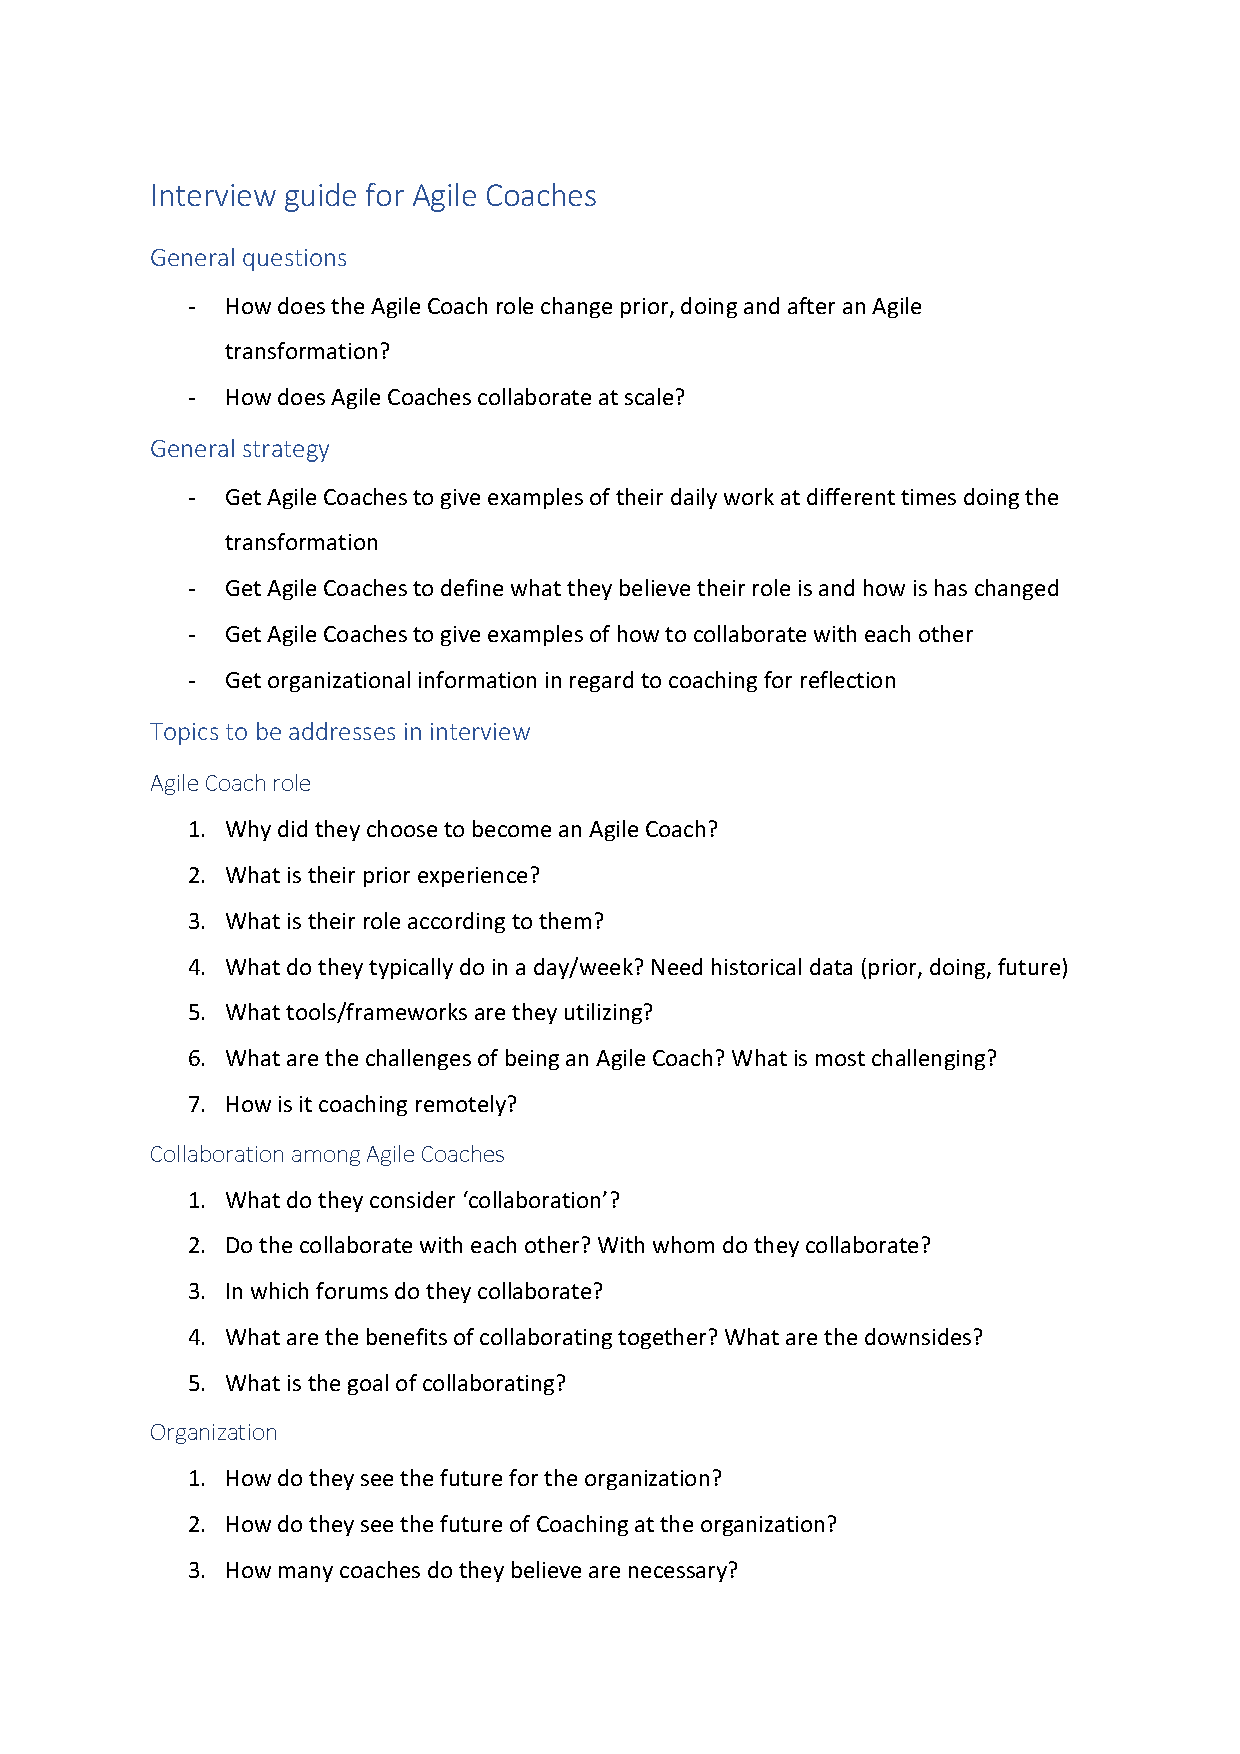
\includegraphics[scale=0.99, page=1]{acInterview.pdf}
\newpage
\includegraphics[scale=1, page=2]{acInterview.pdf}

\restoregeometry
\section{Agile Coach Chapter Lead}
\label{acCLInterviewTemplate}
\newgeometry{top=0in,bottom=0in,right=0in,left=0in}
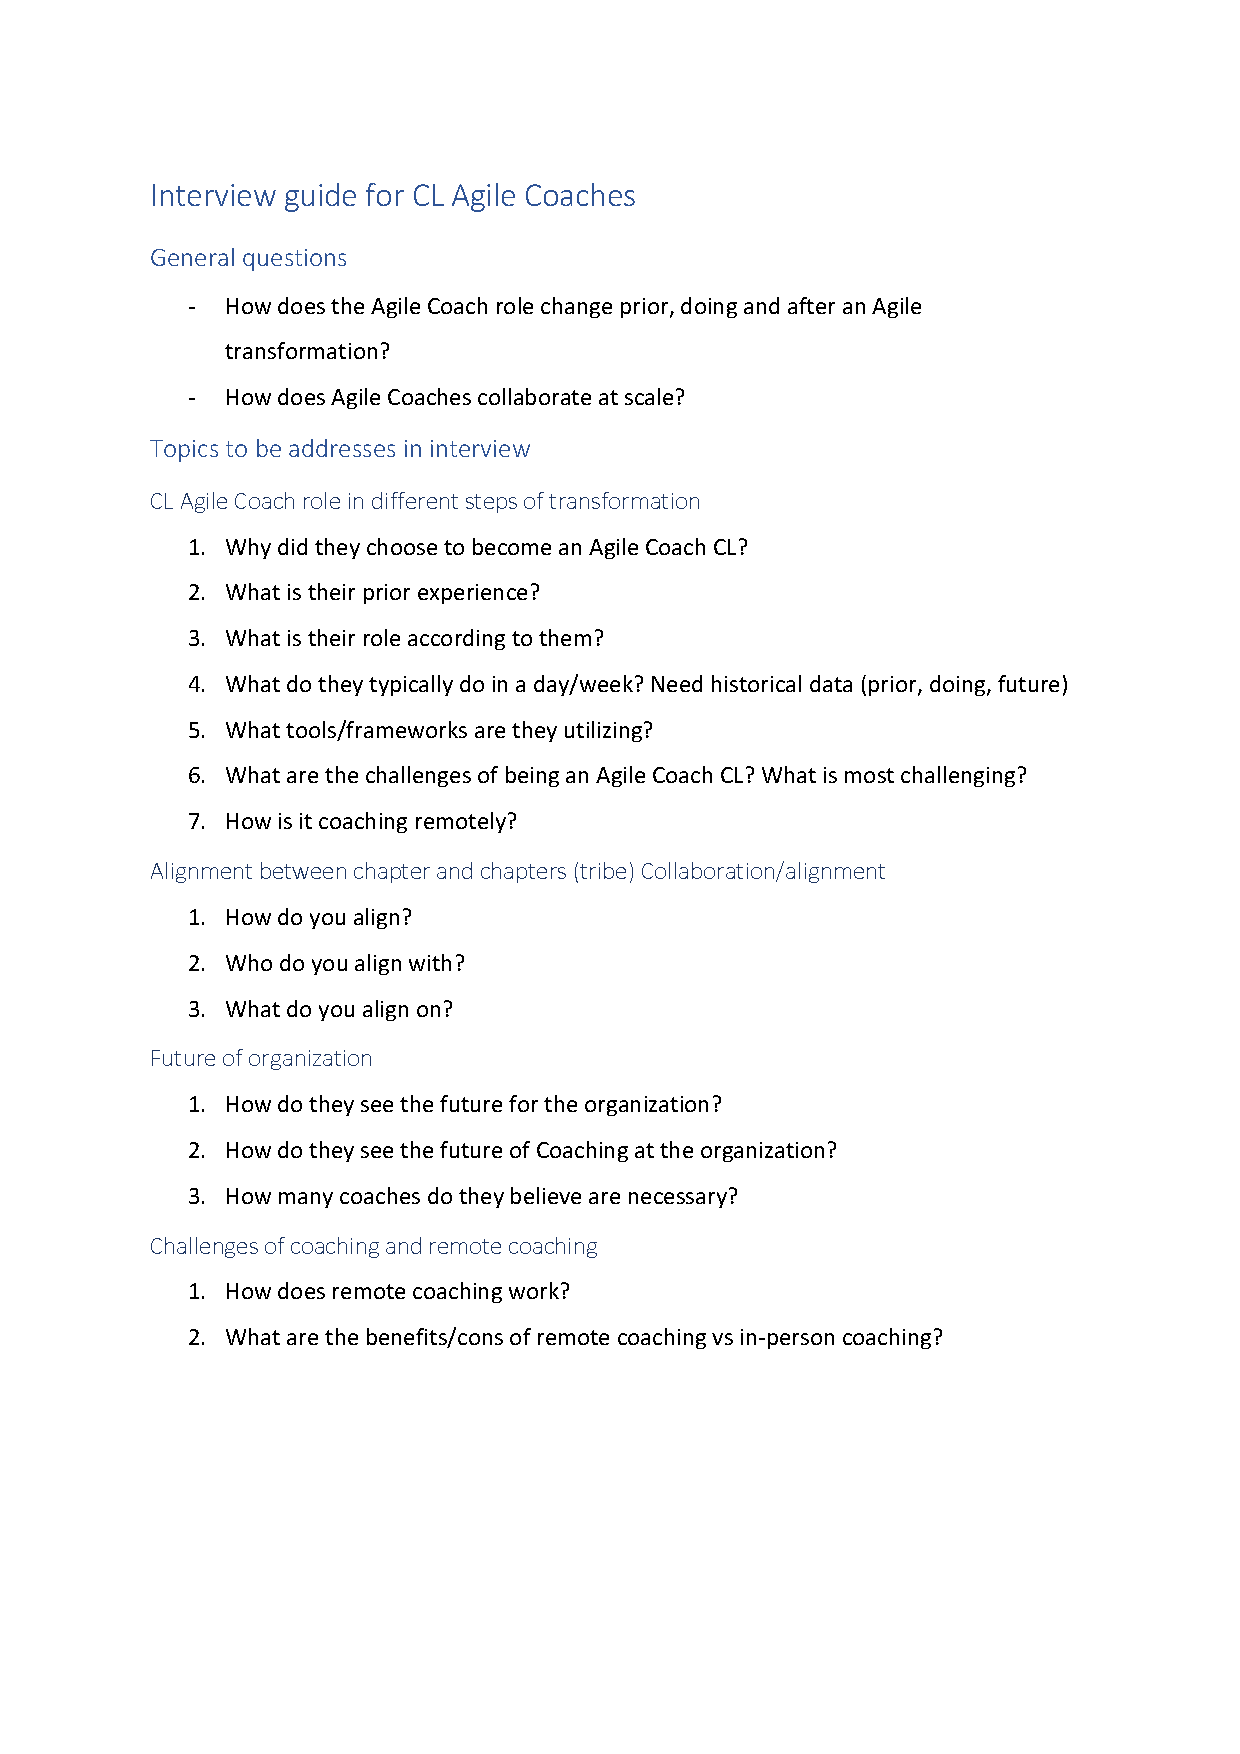
\includegraphics[scale=0.99,page=1]{clInterview.pdf}
\newpage
\includegraphics[page=2]{clInterview.pdf}

\end{document}
